%------------------------------------------------------------------------------
% 
\chapter{Real World Knowledge Acquisition Implementation}
\label{chapter:implementation}
%-------------------------------------------------------------------------------
This chapter presents the actual implementation in the system described
in the previous chapters (especially in \autoref{chapter:approach}). While up 
to now we've been describing the idea and a general approach to do it 
(independent of the implementation), here we represent the actuall working
system that we implemented and kept it online in the shape of the current 
version since the end of 2012. 

During this time, 5,185 users installed its
client app, out of which 2,401 users registered, and 1,715 users used it at 
least once (see the results chapter, \autoref{section:stickiness} for more 
details on users).
The development started on October 26th, 2010 and halted on June 2014. The
implementation follows closely the architecture presented on 
\autoref{fig:Architecture} in \autoref{chapter:approach}. For the core
of the system we took Cyc with its common sense KB and inference engine, which 
was also an initial inspiration for the development and the approach, where
the main work needed to be done on the part of the meta-KB and also common
sense KB extensions to support our use-cases. For the NL modules, our 
implementation relies on the internal Cyc logic to NL conversion modules, and
on SCG\parencite{Schneider2015}. The procedural component and client were 
written from scratch. All together our implemented system consists of 50,686
lines of Java source code, and 12,616 lines of knowledge definitions (8,571) for
the additional knowledge we added in CycKB to drive our KA process.

Besides the implementation described here, this system was also implemented and
deployed as a real-time commuting companion\parencite{Figueiras2013}, and as an
RDF framework for on the field sensor information knowledge acquisition
\parencite{Bradesko2012a}. Commuting companion implementation and this implementation
were also described in the books \emph{Intelligent Decision Technology 
Support in Practice}\parencite{Costa2016} and \emph{Handbook of Human 
Computation}\parencite{Witbrock2013}. This implementation was also mentioned
in the \emph{Communications of the ACM} magazine article\parencite{Geller2016}.

Implementation consists of Android based mobile client, Java Servlet based
\emph{Procedural Component} with PostGreSQL database access, two Cyc instances 
(KB, Inference Engine, NL Conversion) to increase the speed and reliablility 
of the system, \emph{Transcript Server} for syncing between Cyc instances, 
and a web-site for registration and email confirmation. This organization is 
also depicted on \autoref{fig:implementation} below.

\begin{figure}[htb]
	\centering
		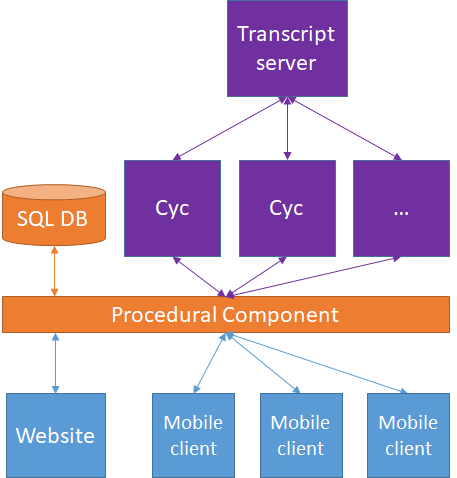
\includegraphics[width=0.7\textwidth]{figures/implementationOrg.png}
	\caption{Organization of the system modules in our implementation.}
	\label{fig:implementation}
\end{figure}


\section{Cyc}
\label{section:Cyc}

TBW

\subsection{SCG}
\label{section:scg}
TBW

\section{Mobile Client}
\label{section:app}
TBW
